\chapter{Implementation}
\label{ch:implementation}

This chapter explains how the simulation was designed to give users a realistic sense of what it might feel like to experience hallucinations, as reported by people living with schizophrenia. The goal was to make the experience both immersive and educational—helping users not only understand the symptoms, but also feel more empathy for those who live with them. The following sections describe how the auditory and visual elements were created, why they were chosen, and what challenges arose during implemetation.

\section{Structure of the Simulation}

The simulation was intentionally structured to create an increasingly unsettling experience that mirrors hallucinations commonly reported in schizophrenia. This design was informed by both clinical research on psychotic symptoms and educational approaches shown to foster empathy and reduce stigma among healthcare professionals.

The auditory hallucinations included in the simulation are modeled after established training tools like Patricia Deegan’s “Hearing Voices” program, which has been shown to significantly enhance empathy in both students and clinicians \cite{Hsia2022}. Building on this model, the simulation presents a series of whispered voices and confrontational phrases. These sounds are introduced gradually and increase in emotional intensity over time, reflecting research that shows emotional engagement enhances learning and empathetic understanding \cite{Skoy2016}.

In addition to auditory elements, the simulation incorporates visual hallucination features. These include colored dots that appear, spatial distortions like dark stains, and a darkening of the visual field. These visual effects were inspired by clinical reports of hallucinations in schizophrenia, which often describe geometric patterns and distorted or symbolic images \cite{Silverstein2021,Vanommen2019}.

The overall structure is designed to simulate both subtle and intense hallucinatory experiences. Initial symptoms—such as whispers and the darkening of the visual field—represent the early stages of changes. As the simulation progresses, the intensity of both auditory and visual elements increases to reflect the overwhelming nature of more severe psychotic episodes. This progression helps users understand how hallucinations can escalate over time and provides insight into the lived experience of individuals with schizophrenia.

\emph{Note: Include the sequence of the simulation here?}

\section{Implementation of the Simulation}

Before diving into the details of how individual components work, it is helpful to understand how the entire simulation is structured and coordinated. The simulation was developed in the Unity game engine, which provided the real-time rendering and interaction environment needed for an immersive experience. However, the core logic of the simulation was implemented through a set of custom C\# scripts, each responsible for specific components of the experience. The system is made up of several different scripts that control what the user sees and hears—from floating dots and stains to whispering voices. To make the experience feel immersive and believable, all of these effects need to happen at the right time and in the right order. This is where the central orchestrator comes in. The following sections explain how the simulation is timed and controlled, starting with the main orchestration logic that acts as the controller of the experience.

\subsection{Orchestration}
At the heart of the system lies the \texttt{Orchestrator.cs} script. This script sequences the entire simulation, controlling when sounds play, visual hallucinations appear, and environmental effects occur. The timeline was structured using IEnumerator coroutines, allowing asynchronous timed execution of events, ensuring immersive pacing without overwhelming the user too early in the experience.

\begin{lstlisting}[language=C++, caption={Orchestration Coroutine}, label={lst:orchestration}]
    IEnumerator OrchestrationSequence()
    {
        Debug.Log("Simulation started");
        yield return new WaitForSeconds(60f);
        PlayWhispers();
        // visual field is getting darker
    
        yield return new WaitForSeconds(5f);
        soundManager.PlaySound("1");
    }
    \end{lstlisting}
    

Synchronization across components ensures the user is not overwhelmed with concurrently being stimulated. For example, whispers begin before visuals, allowing users to acclimate to auditory disturbances before confronting the more visual hallucinations. Those are also paced in relation to the voice samples, building tension across the timeline.
The orchestrator also manages the timing of the visual effects, ensuring that they are introduced at appropriate intervals to create a sense of progression. The following diagram \ref{fig:orchestrator_diagram} illustrates the high-level structure of this system and the flow of variable dependencies among its components.

\begin{landscape}
\begin{figure}[p]
\centering
\begin{tikzpicture}[scale=0.8, transform shape,
  node distance=1.6cm and 2.8cm,
  roundnode/.style={circle, draw=black, fill=black!90, text=white, minimum size=1.2cm},
  purplenode/.style={ellipse, draw=black, fill=purple!20, minimum height=1.2cm, minimum width=1.8cm, align=center},
  yellownode/.style={rectangle, draw=black, fill=yellow!80, rounded corners, align=center, text width=3cm},
  every node/.style={font=\small}
]

% Central node
\node[roundnode] (orchestrator) {Orchestrator};

% Modules

\node[purplenode, above=of orchestrator] (soundmanager) {Sound Manager};
\node[purplenode, left=of orchestrator] (backgroundaudio) {Background Audio};
\node[purplenode, right=of orchestrator] (stains) {Stains};
\node[purplenode, below=of orchestrator] (dotmanager) {Dot Manager};

% Properties

\node[yellownode, above=of soundmanager] (audiosource) {Audio Source};
\node[yellownode, left=of soundmanager] (identifier) {Identifier};

\node[purplenode, above=of identifier] (darkenscreen) {Darken Screen};
\node[yellownode, left=of darkenscreen] (darkpanel) {Dark Panel};
\node[yellownode, above=of darkenscreen] (fadeduration) {Fade Duration};

\node[yellownode, left=of backgroundaudio] (whispers) {Whispers};

\node[yellownode, above=of stains] (numstains) {Number of Stains};
\node[yellownode, above right=of stains] (spawnradius) {Spawn Point, Radius};
\node[yellownode, right=of stains] (spawninterval) {Spawn and Disappearance Interval};
\node[yellownode, below=of stains] (sphereprefab) {Sphere Prefab};


\node[yellownode, below=of dotmanager] (numdots) {Number of Dots};
\node[yellownode, right=of dotmanager] (dotprefab) {Dot Prefab};
\node[yellownode, left=of dotmanager] (spawnarea) {Spawn Width, Height, Depth};
\node[yellownode, right=of dotprefab] (collisionhandling) {Collision Handling};
\node[yellownode, below=of collisionhandling] (collisioneffect) {On Collision Enter \\ $\Rightarrow$ Color Change};


% Connections
\draw (orchestrator) -- (soundmanager);
\draw (orchestrator) -- (backgroundaudio);
\draw (orchestrator) -- (stains);
\draw (orchestrator) -- (dotmanager);

\draw (darkenscreen) -- (darkpanel);
\draw (darkenscreen) -- (fadeduration);


\draw (soundmanager) -- (audiosource);
\draw (soundmanager) -- (identifier);

\draw (backgroundaudio) -- (whispers);

\draw (stains) -- (numstains);
\draw (stains) -- (spawnradius);
\draw (stains) -- (spawninterval);
\draw (stains) -- (sphereprefab);
\draw (dotprefab) -- (collisionhandling);
\draw (collisionhandling) -- (collisioneffect);

\draw (dotmanager) -- (numdots);
\draw (dotmanager) -- (dotprefab);
\draw (dotmanager) -- (spawnarea);


\end{tikzpicture}%

\caption{System architecture and variable orchestration for MR schizophrenia simulation.}
\label{fig:orchestrator_diagram}
\end{figure}
\end{landscape}


\subsection{Auditory Hallucinations}

Auditory hallucinations in the simulation are managed by the \texttt{SoundManager.cs} script, which handles the playback of voice samples that simulate inner voices or intrusive thoughts. These sounds are intended to create an immersive and unsettling auditory environment that reflects commonly reported auditory hallucination experiences.

The core logic of the script is based on a list of \texttt{AudioSourceConfig} objects, each of which includes an \texttt{AudioSource} and a corresponding string identifier called \texttt{voiceGroup}. This was initially thought to be the identifier per voice, but as it became apparant that the script needs to follow a certain sequence, the identifier was stricly for knowing which section to play. Therefore, the script was divided into 12 parts, such that it could be controlled which part of the script should be played when. 

Upon initialization, the script constructs a mapping of each voice group identifier to its respective audio source. When the method \texttt{PlaySound(string voiceGroup)} is called, the corresponding audio source is checked to ensure it is not already playing—this prevents overlapping audio playback. If no sound is currently playing for that identifier, the audio clip is played and logged for debugging purposes. If the requested identifier is not found, an error is reported.

\vspace{1em}
The actual audio content was carefully scripted to reflect a broad emotional spectrum, ranging from ambiguous or confused statements to more aggressive or paranoid lines. These phrases were written in French—the working language of the institution—and designed to evoke discomfort and mostly distraction. To achieve a very natural tone of the voices, the voices were generated using the ElevenLabs text-to-speech AI platform \cite{elevenlabs}, where voices can be created with specific promps. The prompts therefore instructed the AI platform to create a voice which was primarly scared, one which was whispering, and one which was more aggressive. The goal was to create a range of voices that could be used to simulate different types of auditory hallucinations, from soft whispers to more confrontational tones.

The voice samples were not developed in isolation. Their emotional tone, content, and perceived realism were refined through close collaboration with the \textit{Haute école de santé Fribourg} (HEdS-FR). We reviewed the script with faculty members experienced in mental health care. Their feedback directly influenced the final selection of voice lines, ensuring that the content remained as truthful as possible. 

\vspace{1em}
The final script used in the simulation is shown in Table~\ref{tab:audio_script}, presented in both the original French and their English translations.

\begin{table}[H]
\centering
\begin{tabular}{|p{7cm}|p{7cm}|}
\hline
\textbf{Français (Original)} & \textbf{English (Translation)} \\
\hline
Écoute c’que dit l’enseignant & Listen to what the teacher says \\
Écoute attentivement. & Listen carefully. \\
Est-ce que t’entends ça ? & Do you hear that? \\
Tu connais la réponse ? & Do you know the answer? \\
Bien sûr que tu n’la connais pas & Of course you don’t know it \\
T'es vraiment stupide. & You're really stupid. \\
Tu n’sers à rien & You're useless \\
Tu vois les autres ? & Do you see the others? \\
Ils parlent de toi. & They're talking about you. \\
Fais attention à toi. & Watch out. \\
Ne leur fais pas confiance. & Don't trust them. \\
Quelles sont ces taches ? & What are those stains? \\
Tu vois ça ? & Do you see that? \\
Concentre-toi ! & Focus! \\
Les autres te regardent. & The others are watching you. \\
Tu n’le vois pas ? & You don’t see it? \\
Regard vers le haut. Ya quelque chose ! & Look up. There's something there! \\
Regarde maintenant ! & Look now! \\
Qu’est-ce qui n’va pas chez toi ? & What’s wrong with you? \\
Tu n’vaux rien & You’re worthless \\
Touche les points ! & Touch the dots! \\
Les autres veulent enregistrer tes pensées. & The others want to record your thoughts. \\
Tu dois faire attention ! & You must be careful! \\
Regarde derrière toi ! & Look behind you! \\
Fais attention ! & Be careful! \\
Tu dois faire attention à toi ! & You must look after yourself! \\
\hline
\end{tabular}
\caption{French simulation script with English translation}
\label{tab:audio_script}
\end{table}

\vspace{1em}
To further enhance immersion, the timing of the voice playback is synchronized with corresponding visual effects, such as the appearance of stains or the darkening of the screen. This multisensory coordination aims to simulate the overwhelming and often unpredictable nature of psychotic episodes. The flexible structure of the \texttt{SoundManager.cs} makes it possible to easily add, remove, or sequence new voices for future versions of the simulation.

\subsection{Visual Hallucinations}

The simulation includes several visual effects designed to represent different kinds of hallucinations, based on how people with schizophrenia have described their experiences. 

\subsubsection{Screen Darkening}

The screen darkening effect in the simulation is implemented via the \texttt{ScreenDarkener.cs} component, which gradually overlays a semi-transparent black panel onto the user's visual field. This visual modification simulates a sense of tunnel vision or visual deterioration, contributing to the immersive experience of altered perception.

Technically, the effect is realized through a full-screen \texttt{Image} component referred to as \texttt{darkPanel}. This panel is a background panel from Unity itself with the color set to black. We can nicely see the panel in the Unity scene in figure \ref{fig:darkpanel}. 

\begin{figure}[h!] 
    \centering 
    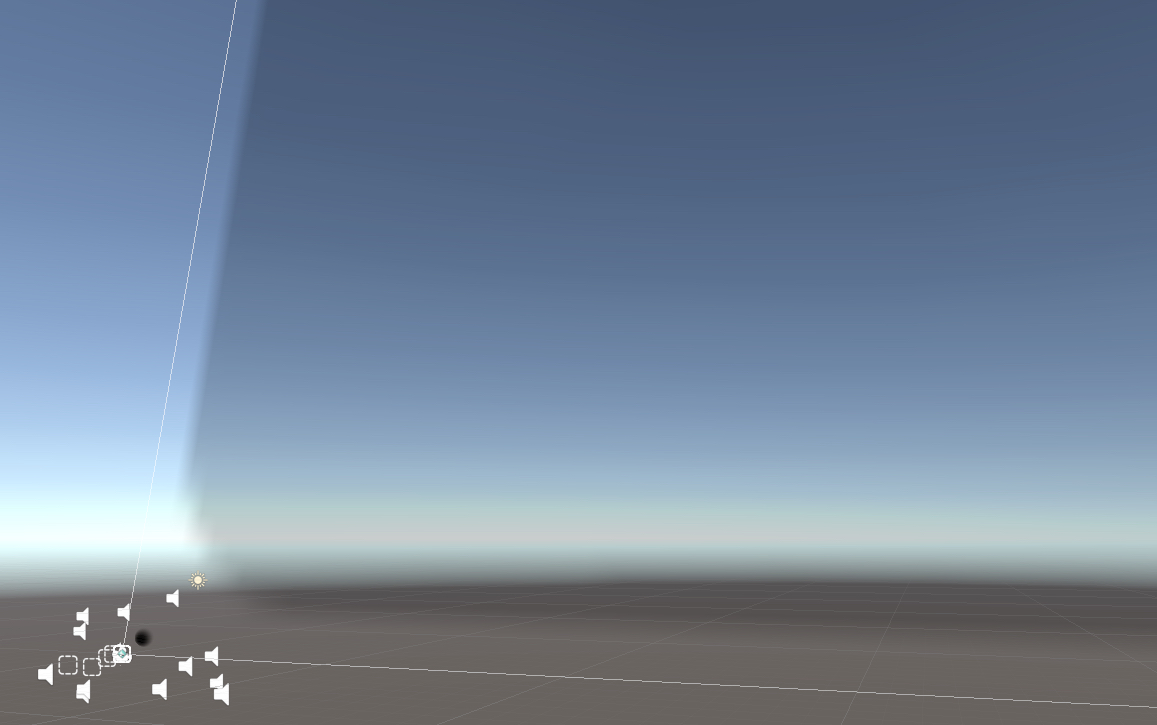
\includegraphics[width=0.8\textwidth]{../../Figures/darkpanel.jpg} 
    \caption{Dark background panel to mimic darkening of the user's visual field} 
    \label{fig:darkpanel} 
\end{figure}

At the start of the simulation, the alpha value of this panel is set to zero, ensuring that the screen appears completely transparent and preventing any initial visual flash. With the start of the simulation a coroutine is triggered that increases the panel’s alpha value from 0 to 0.7 over a duration which can be set in Unity itself, called the (\texttt{fadeDuration}, typically 2 seconds).

The darkening culminates in a panel opacity of 70\% (i.e., \texttt{alpha = 0.7}), which darkens the screen significantly without making it fully dark. This design choice maintains visibility while still inducing a sense of discomfort or visual strain. As such, the effect models subtle visual hallucinations or perceptual narrowing, which are commonly reported in psychotic experiences. 

\subsubsection{Stains}
One effect, created using the \texttt{DynamicWaveDeformation.cs} script, makes the surfaces of objects appear to ripple and shift. This gives them a wavy, moving look that reflects how perception can feel distorted during hallucinations. This deformation was applied to spheres which are triggered by a pre-defined spawn and disappearance interval. The spheres are randomly placed in the user's field of view, and they float around, creating a sense of visual noise. The \texttt{FadeEdgeShader.shader} shader was used to create a darkening effect around the edges of the screen, simulating the feeling of being in a confined space or having a limited field of vision. This shader was created with the help of ChatGPT, which provided a basic structure that was then customized to fit the specific needs of the simulation.

The \texttt{Orchestrator.cs} script manages when these spheres appear during the simulation timeline. The method \texttt{SpawnSphere()} is invoked repeatedly in a loop to instantiate the spheres at randomized positions around a central \texttt{spawnPoint}. The number of spheres and the interval between their appearances are determined by the parameters \texttt{sphereCount} and \texttt{spawnInterval}, respectively.Each sphere is placed within a circular area defined by a \texttt{spawnRadius}, with its Y-coordinate fixed to match the user’s eye level for spatial consistency. After a fixed delay, the spheres are removed in the same order they appeared, one by one, using a queue-based removal mechanism and the \texttt{Destroy()} function. 

\vspace{1em}

The visual appearance of these spheres is designed to be ambiguous and somewhat unnatural. They show a constantly shifting surface that pulses and distorts as if they are made out of a wavy material to represent stains. This is achieved through the \texttt{DynamicWaveDeformation.cs} script, which displaces the vertices of each sphere's mesh in real time, to create this wave effect.

When oinstantiated, the script stores the original mesh vertices and continuously updates them every frame based on the wave function that combines sine and cosine operations on both the X and Z components of each vertex:

\begin{quote}
\texttt{float wave = sin(time + x) * cos(time + z)}
\end{quote}

The wave value is multiplied by a configurable strength parameter called \texttt{waveAmplitude}, and this result is used to slightly move each point on the sphere’s surface outward or inward along its normal direction. This creates a rippling effect across the whole object, making the sphere appear as if it is softly pulsing or "breathing" while it exists in the environment.


\paragraph{Visual Example}
Figure~\ref{fig:stain} shows a black deforming sphere as it appears in the real-world mixed reality classroom context. The shader used for this object includes a soft fade around the edges, giving it a non-solid, ghostly appearance that blends slightly with the background. Figure~\ref{fig:fadeedgeshader} illustrates the same object in the Unity Editor, where the mesh deformation and alpha transparency are more clearly visible.


\begin{figure}[h!] 
    \centering 
    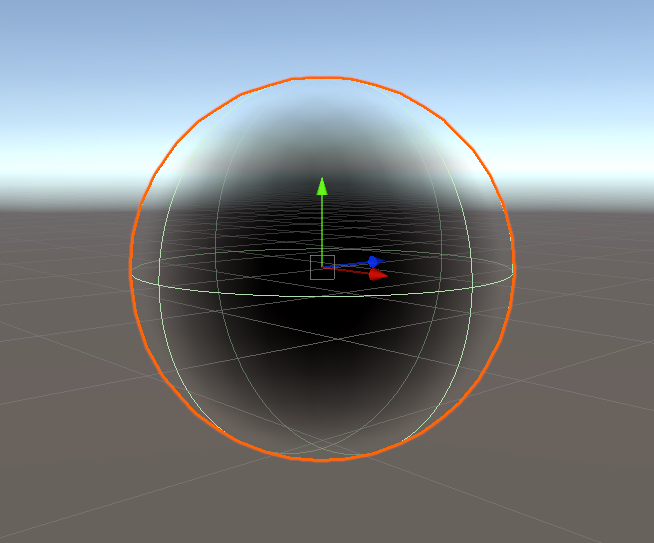
\includegraphics[width=0.6\textwidth]{../../Figures/fadeedgeshader.jpg} 
    \caption{Example sphere with the \texttt{FadeEdgeShader.shader} and the \texttt{DynamicWaveDeformation.cs} script to mimic stains} 
    \label{fig:fadeedgeshader} 
\end{figure}

\begin{figure}[h!] 
    \centering 
    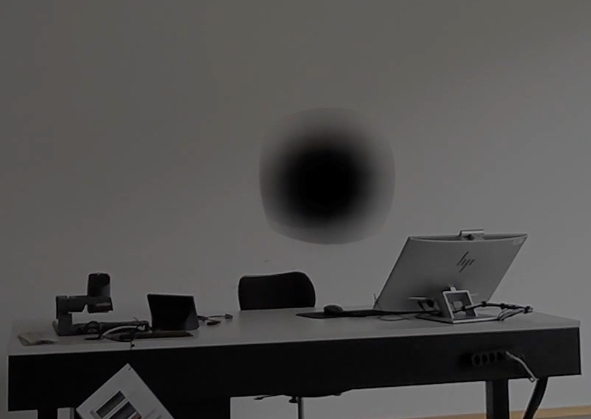
\includegraphics[width=0.6\textwidth]{../../Figures/stain-video.jpg} 
    \caption{Stain appearing in the user's field of view} 
    \label{fig:stain} 
\end{figure}

\subsubsection{Floating Dots and Interaction Logic}

To help simulate the kind of perceptual disturbances that some people with psychosis experience, the simulation includes floating colored dots that the user can interact with. These are controlled by two main scripts: \texttt{DotManager.cs}, which creates the floating dots, and \texttt{ObjectCollision.cs}, which handles what happens when users touch the interactive spheres.

\vspace{1em}

The \texttt{DotManager.cs} script is responsible for filling the space around the user with a number of small red and blue spheres—referred to as “dots.” These dots are placed randomly within a area, defined by the parameters \texttt{spawnWidth}, \texttt{spawnHeight}, and \texttt{spawnDepth}. To not overcrowd the visual field, the script makes sure that each dot is placed far enough away from the others. If a dot would be too close to a previous one, a new position is chosen.

Each dot is randomly colored red or blue, creating a scattered, noisy effect. The idea is to make the environment feel just a bit off or overwhelming, without making it frightening.The dots are also meant to be more interactive. They appear at different moments in the simulation and are set up to respond when the user reaches out and touches them. The logic behind this is handled by the \texttt{ObjectCollision.cs} script.

Using Unity's collision detection system, the script monitors for \texttt{OnTriggerEnter} and \texttt{OnTriggerExit} events. When the user's hand (or other collider) enters the trigger zone of a sphere, the following actions are executed:

\begin{itemize}
    \item The object's material is changed to a new, randomly generated color using \texttt{Random.ColorHSV()}. This signals to the user that the object has responded to their touch.
    \item The script searches the scene for an \texttt{AudioSource} tagged as \texttt{"Audio10"} and stops it using \texttt{audioSource.Stop()}. This source plays a looping sound \textit{"Touche les points !"} (Touch the dots!), intended to mimic intrusive auditory hallucinations. Its termination represents a temporary sense of relief or control.
\end{itemize}

The interaction is simple but meaningful. It represents how some people try to manage or quiet their hallucinations—by focusing on them or interacting in some way. In the simulation, this also makes the experience more engaging and lets users take an active role, rather than just being passive observers.

\paragraph{Visual Example}
The images below illustrate the interaction process. In Figure~\ref{fig:dots_before}, the user sees floating dots in their original red and blue state. After touching a sphere, as shown in Figure~\ref{fig:dots_after}, the affected object changes color, confirming that the interaction was registered and the audio loop was interrupted.

\begin{figure}[H]
    \centering
    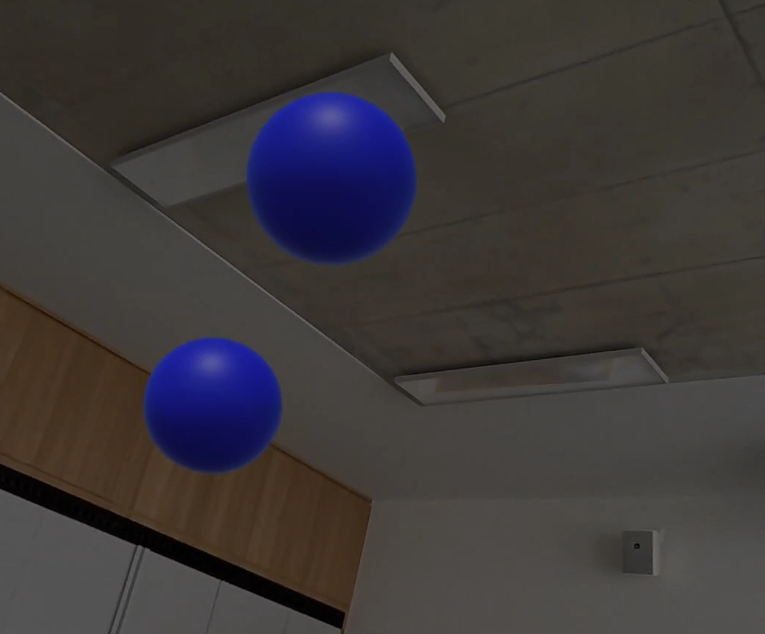
\includegraphics[width=0.6\textwidth]{../../Figures/dots-video.jpg}
    \caption{Floating dots before user interaction.}
    \label{fig:dots_before}
\end{figure}

\begin{figure}[H]
    \centering
    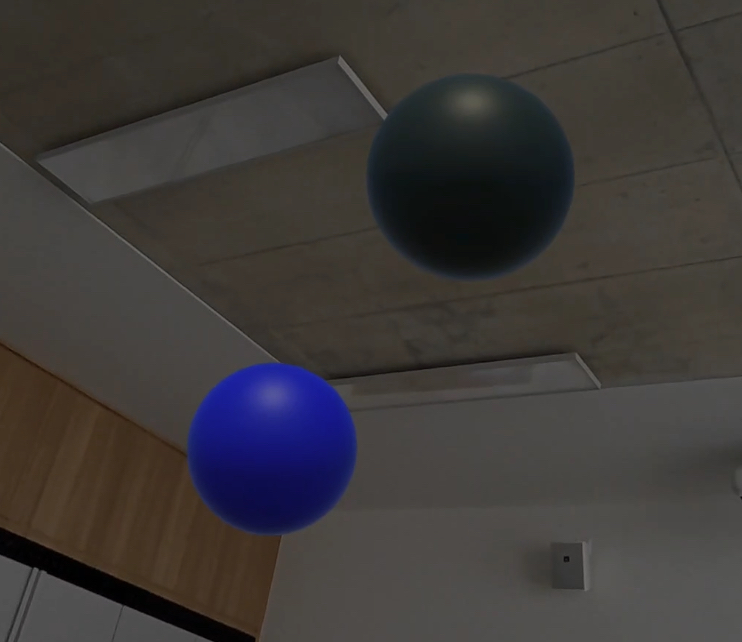
\includegraphics[width=0.6\textwidth]{../../Figures/dots-after-touch.jpg}
    \caption{Color change after user touches one of the dots.}
    \label{fig:dots_after}
\end{figure}


Together, these two systems—floating dots and interactive auditory element of the dots—form a approach to simulating environmental disruption. While the \texttt{DotManager.cs} creates persistent visual distraction, the \texttt{ObjectCollision} system adds intensity. The use of sound looping and the color change of the dots reinforces the themes of intrusion and momentary relief, central to the projects goal of eliciting empathetic insight into the lived experience of a psychosis.


\section{Challenges During Implementation} 
Despite careful planning, several significant challenges emerged during the development of the simulation:

\subsection{Audio Loops} 
Initially, each interactive sphere instantiated its own sound playback. This led to multiple overlapping sound loops, which had to be fixed. The problem arose because the audio logic was not centralized — each sphere's ObjectCollision component independently triggered audio playback upon spawning. For example, if five spheres were instantiated, each would play its own sound, leading to overlapping audio. The audio would then only stop, if all five spheres were touched, which was not the intended behavior.

To solve this issue, a shared audio management system was developed, which is a static AudioSource and coroutine created within \texttt{ObjectCollision.cs}. This means that only one looped sound source exists, and it is globally stopped when a user interacts with any sphere.

A key logic excerpt illustrating this centralization is:

\begin{quote} \small \texttt{if (sharedAudioSource == null) { sharedAudioSource = ...; coroutineHost = this; repeatCoroutine = coroutineHost.StartCoroutine(RepeatAudio());}} \end{quote}

This ensures no duplicate sounds occur, even with multiple spheres present.

\subsection{Finger Interaction} 
A second major challenge was accurately detecting when a user touched a dot. Initially, an additional \textit{poke interaction} module was mistakenly integrated alongside the already built-in collision detection by Unity. This redundant system caused conflicting behavior and unpredictable touch responses. Upon deeper inspection, it was discovered that Unitys hand collision system already assigns specific identifiers to each fingertip collider, such as \textit{HandIndex1} for the index finger. Reliable detection could therefore be implemented simply by checking the collision object's name during a collision event, rather than adding redundant interaction modules.

\begin{quote} \small \texttt{if (collision.gameObject.name.Contains("HandIndex1")) { ... }} \end{quote}

By implementing this and removing the redundant poke interaction, the color changing was a smooth process and the finger identification also worked.

\subsection{Loud Audio} 
During preliminary testing, the built-in speakers of the Meta Quest 3 were found to be too loud, leaking audio to the entire room and were being heard by observers. To address this, PhoneLook bone-conduction headphones\footnote{\url{https://www.phonelook.ch/de/stylische-kabellose-bluetooth-knochenleitungs-kopfhorer-fur-sport-laufen-radfahren-fitness-schwarz.html}} were integrated into the simulation setup. This had the advantage that the audio is transmitted privately to the participant without occluding ambient sounds.
It also ensures immersive simulatin while respecting privacy and the testing environment.

\subsection{Spatial Placement of Audio } 
Another significant challenge was the spatial arrangement of audio sources within the simulation environment. Initially, it was difficult to orient myself correctly in Unityss Scene View, making it unclear where the sounds would originate from relative to the user position. Proper placement was essential to create a convincing spatial auditory experience, because sounds had to feel anchored in specific locations in the environment. As the user moved, the sounds needed to remain fixed in space, enhancing realism and immersion.

To solve this, I invested time to become familiar with Unity's camera controls and 3D scene navigation.Then, the sound sources were distributed strategically across different coordinates, ensuring that different hallucinated voices would come from distinct spatial directions.

An example of the 3D placement of the sound sources in the Unity scene is shown in \autoref{fig:sound_sources}.

\begin{figure}[h!] \centering 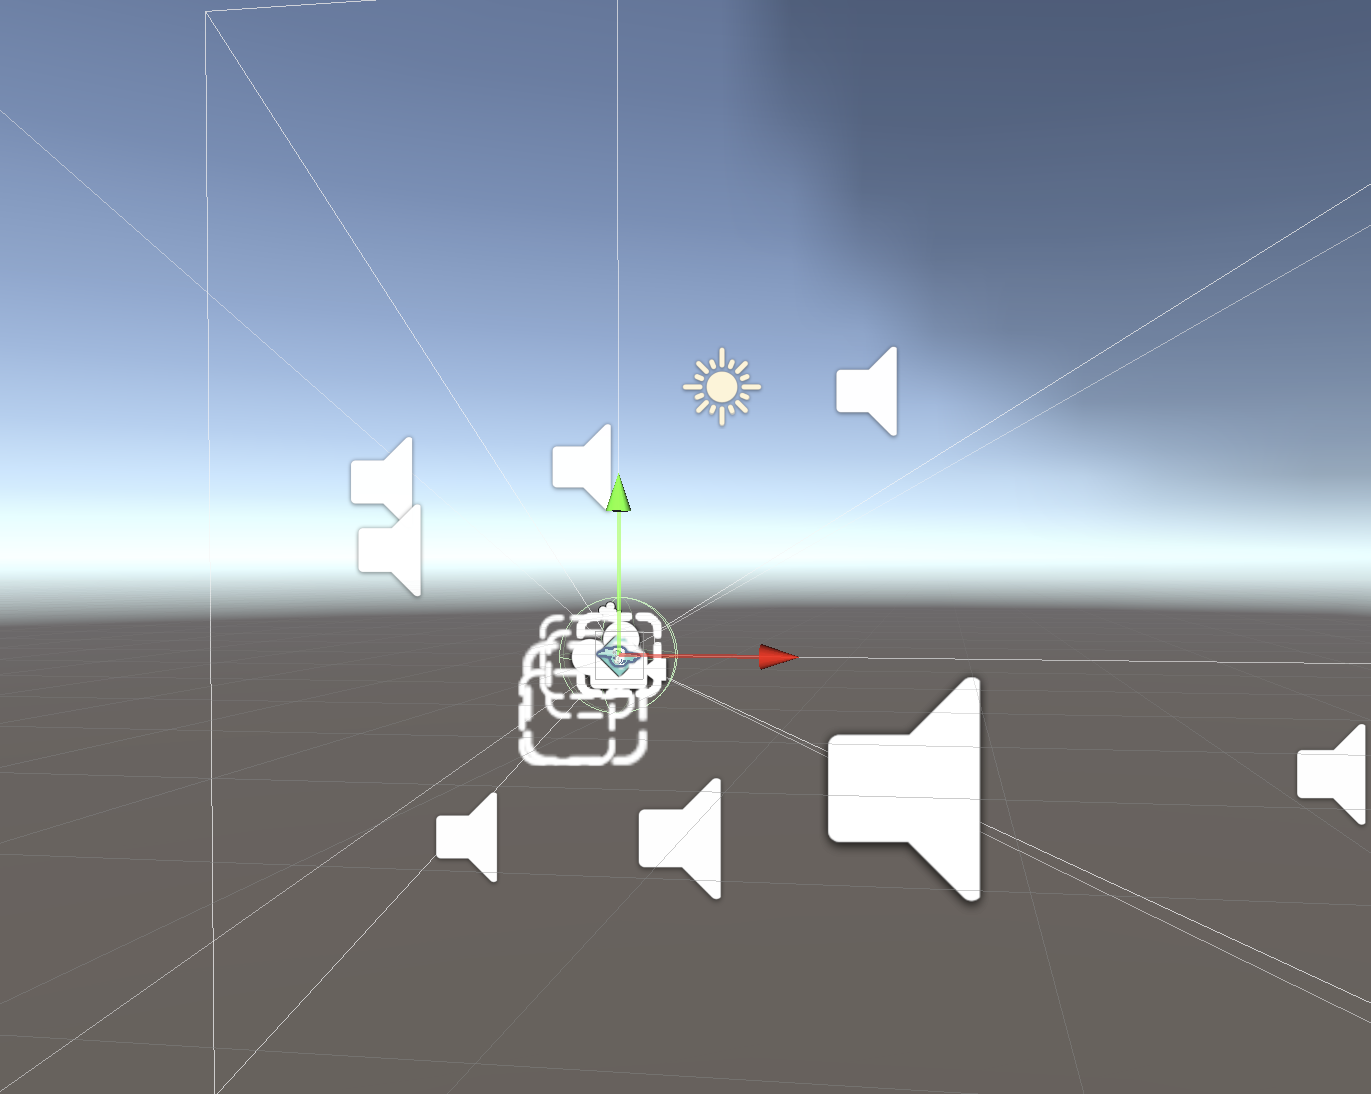
\includegraphics[width=0.8\textwidth]{../../Figures/unity-scene.png} \caption{Placement of spatial sound sources in the Unity scene for the hallucination simulation. Each speaker icon represents a sound source emitting a hallucination voice.} \label{fig:sound_sources} \end{figure}

